\documentclass[]{llncs}
\usepackage{graphicx}

%\documentclass{article}
\usepackage{mathtools}
\usepackage{times}  % DO NOT CHANGE THIS
\usepackage{helvet} % DO NOT CHANGE THIS
\usepackage{courier}  % DO NOT CHANGE THIS
\usepackage[hyphens]{url}  % DO NOT CHANGE THIS
\usepackage{arydshln}
\usepackage{mathptmx}
\usepackage{amsmath}
\usepackage{bm}
\usepackage[english]{babel}
\usepackage[utf8]{inputenc}
\usepackage{algorithm}
\usepackage{epstopdf}
\usepackage{booktabs}
\usepackage{multirow}
\usepackage{siunitx}
\usepackage{rotating}
\usepackage{hyperref}
\usepackage[utf8]{inputenc}
\usepackage[T1]{fontenc}
\usepackage{mathtools}
\usepackage[thinc]{esdiff}
%\usepackage[algo2e]{algorithm2e}
%\usepackage{arevmath}     % For math symbols
\usepackage[noend]{algpseudocode}
\urlstyle{rm} % DO NOT CHANGE THIS
\def\UrlFont{\rm}  % DO NOT CHANGE T
% Used for displaying a sample figure. If possible, figure files should
% be included in EPS format.
%
% If you use the hyperref package, please uncomment the following line
% to display URLs in blue roman font according to Springer's eBook style:
% \renewcommand\UrlFont{\color{blue}\rmfamily}

\pagestyle{plain}
\setcounter{page}{1}
\pagenumbering{arabic}

\DeclareMathOperator {\argmax}{argmax} 

\begin{document}

\title{Adaptive Dynamics for the Direct Actions Strategy Approach}

\author{Frances Cameron-Muller, Supervisor: Dr. Julian Garcia}

\institute{Monash University}

\maketitle    

\section{Adaptive Dynamics for Once Off Stag Hunt Game}

Let $x_i \in [0,1]$ be the probability that agent i cooperates. \\
The Stag Hunt Payoff matrix is 
\[
  \begin{pmatrix} 
   R & S  \\
   T & P  
   \end{pmatrix} 
\]
with $ R > T \geq P > S $ \\
\\
Let $ \Pi ( y, x_{-} )$ be the payoff function of playing a strategy y against the rest of the population playing the strategy x. 
\[
\Pi ( y, x_{-} ) = R x y + S (1-x) y +  T x (1-y) + P (1-x) (1-y)
\]
\\
The invasion fitness of a rare mutant strategy y in a population that consists of only strategy x is given by 
\[
f_x(y) = \Pi ( y, x_{-} ) - \Pi ( x, x_{-} )
\]
\begin{multline}
f_x(y) = R x y + S (1-x) y +  T x (1-y) + P (1-x) (1-y) \\ - R x^2 - S (1-x) x - T x (1-x) - P (1-x) (1-x)
\end{multline}
\[
D(x) = \diffp*{f_x(y)}{y}{y=x}
\]
\[
D(x) = (R - S - T +P) x + (S-P)
\]
\\
Let $H = \frac{P-S}{R - S - T +P} $ also known as the threshold with $ D(H) = 0 $.\\
\\
For $x < H, D(x) < 0$ and for $x > H, D(x) > 0$
This means that for x values below the threshold, the best payoffs are achieved by decreasing the value of x and converging to the Nash equilibrium of always defecting and for x values above the threshold, the best payoffs are achieved by increasing the value of x and converging to the Nash equilibrium of always cooperating. 

\subsection{Example}

Consider a model with dominant strategy $x = 0.1$ interpreted as agents will only cooperate in 10\% of games and a rare mutant strategy $y = 0.7$ representing agents will cooperate in 70\% of games. 
\[
   \text{Payoff Matrix} = \begin{pmatrix} 
   6 & 1  \\
   3 & 2  
   \end{pmatrix} 
\]
The invasion fitness of the rare mutant strategy y = 0.7 is 
\begin{multline}
f_{0.1}(0.7) = 6 0.1 0.7 + 1 (1-0.1) 0.7 +  3 0.1 (1-0.7) + 2 (1-0.1) (1-0.7) \\ - 6 0.1^2 - 1 (1-0.1) 0.1 - 3 0.1 (1-0.1) - 1 (1-0.1) (1-0.1) = 0.45
\end{multline}
The strategy has a positive invasion fitness.
\[
D(x) = D(0.1) = (6 - 1 - 3 +2) 0.1 + (1-2) = -0.6
\]
Since the partial derivative is negative this suggests that the current dominant belief of $x = 0.1$ should be increased. 


\section{Adaptive Dynamics incorporating the Alpha Paramter}

Now let's introduce a new parameter $\alpha \in [0, 1]$ where $\alpha$ is the probability that an agent is matched to play against a copy of themselves instead of their original opponent. 
\\
Therefore, the expected payoff is given by the sum of payoffs of when an agent plays their copy and when an agent plays their original opponent, weighted by the probabilities.
\[ 
\Pi ( y, x_{-}, \alpha ) = \alpha \Pi ( y, y) + (1-\alpha) \Pi ( y, x_{-} )
\]
The new invasion fitness of a rare mutant strategy y in a population that consists of only strategy x is given by 
\[
f_x(y) = \Pi ( y, x_{-}, \alpha ) - \Pi ( x, x_{-}, \alpha )
\]
\[
f_x(y) = \alpha \Pi ( y, y) + (1-\alpha) \Pi ( y, x_{-} ) - \alpha \Pi ( x, x) - (1-\alpha) \Pi ( x,  x_{-} )
\]
\[
f_x(y) = \alpha \Pi ( y, y) + (1-\alpha) \Pi ( y, x_{-} ) - \Pi ( x,  x_{-} )
\]
\begin{multline}
f_x(y) = \alpha (R-S-T+P) y^2 +(S + \alpha T - P - \alpha P) y + (1-\alpha) (R-S-T+P) x y \\+ (-\alpha T + \alpha P - S + P) x + (-R+S+T-P) x^2
\end{multline}
\[
D(x) = \diffp*{f_x(y)}{y}{y=x}
\]
\[
D(x) = (1+\alpha) (R-S-T+P) x + (S + \alpha T - P - \alpha P) 
\]
\[
H = \frac{S + \alpha T - P - \alpha P}{(1+\alpha)(R-S-T+P)}
\]

\section{Graphs}
The derivative of the invasion fitness function of a rare mutant strategy, D(x), is graphed below for all possible dominant strategies, x $\in [0,1]$. Negative values of D(x) indicate the best payoffs are achieved by decreasing the value of x whereas for positive values of D(x), greater payoffs are achieved by increasing x. The function D(x) was graphed for two different payoff matrices [4,1:3,2] and [6,1;3,2]. This shows how the invasion fitness of a rare mutant strategy is impacted by the relative difference in the payoffs between cooperating and defecting. The graph below shows that when the payoff for cooperating is much greater than the payoff for cooperating, the threshold at which D(x) changes sign occurs at a smaller value of x. This demonstrates that greater relative payoffs for cooperation increase the probability of social cooperation as rare mutant strategies are more likely to increase the dominant strategy. This behaviour was observed in the simulation results. 

\begin{figure}
\centering
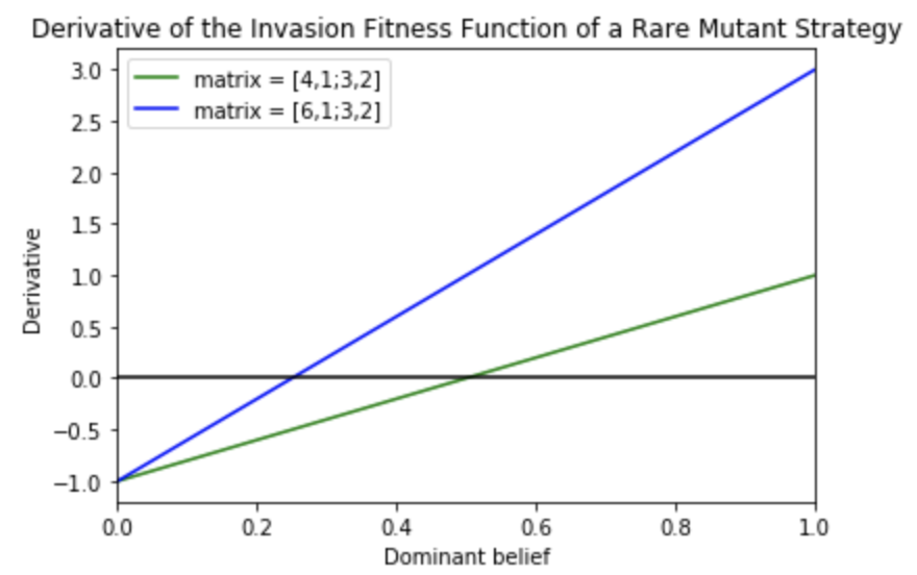
\includegraphics[width=12cm]{images/invasion_fitness}
\end{figure}

The second graph shows the same function as the graph above, the derivative of the invasion fitness function of a rare mutant strategy, D(x), when we incorporate the parameter, alpha. The graphs shows D(x) for the same payoff matrix [4,1;3,2] but for three values of alpha. When alpha = 0, meaning the  probability that an agent is matched to play against a copy of themselves instead of their original opponent is zero, we observe the exact same function in the previous graph, as expected. When alpha = 1, D(x) is always positive illustrating that the agents learning to cooperate is always achieved if the agents are only playing against a copy of themselves. For alpha values between 0 and 1, as alpha increases the threshold for D(x) decreases. Therefore, the more likely the agents are to play against opponents that are similar to themselves, the more likely they will learn to cooperate. 

\begin{figure}
\centering
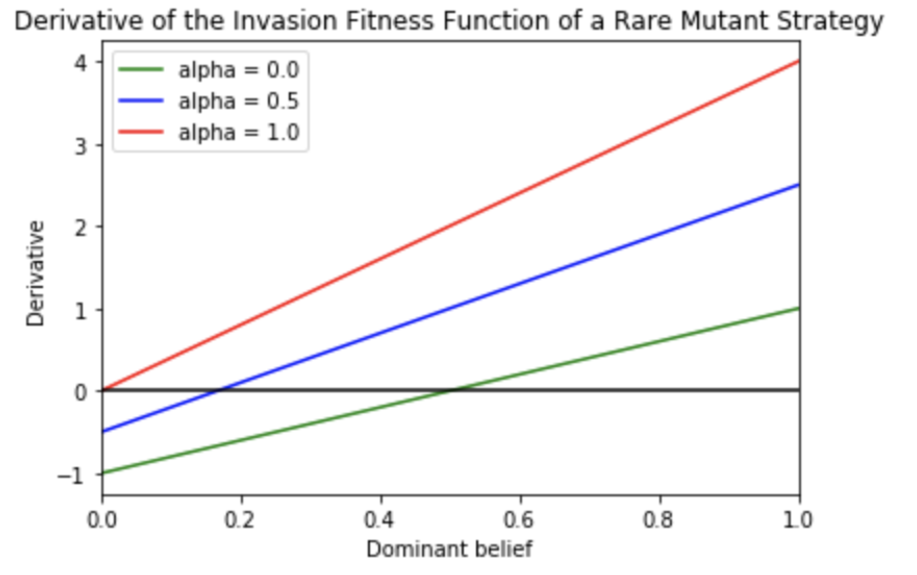
\includegraphics[width=12cm]{images/invasion_fitness_alpha}
\end{figure}


\section{Extending to Ingroup and Outgroup Strategies}

\subsection{Once Off Stag Hunt}

Each agent in the population has a two-dimensional strategy profile strategy, $x_i$, consisting of an ingroup and outgroup strategy,  $x_i = (x_{in}, x_{out})$\\
\\
$x_{in} \in [0,1]$ is the probability that an agent with a strategy profile x cooperates with an individual from the ingroup. \\
\\
$x_{out} \in [0,1]$ is the probability that an agent with a strategy profile x cooperates with an individual from the outgroup. \\
\\
Let $\beta_i \in [0,1]$ be the probability that agent i plays an individual from the ingroup.\\
\\
Let $\beta_{-i} = 1 -\beta_i $ be the probability that an agent of the opposite group of agent i plays an individual from the ingroup.\\

Let $ \Pi ( y, x_{-}, \beta_y)$ be the payoff function of playing a strategy $y = (y_{in}, y_{out}) $ against the rest of the population playing the strategy $x = (x_{in}, x_{out})$ where the probability of an agent playing the strategy y matching with an individual from the ingroup is $\beta_y$.
\[
\Pi ( y, x_{-} , \beta_y) = \beta_y \Pi ( y_{in}, x_{in}) + (1-\beta_y) \Pi ( y_{out}, x_{out} ) 
\]
\\
The invasion fitness of a rare mutant strategy y in a population that consists of only strategy x is given by 
\[
f_x(y) = \Pi ( y, x_{-} , \beta_y) - \Pi ( x, x_{-} , \beta_x) 
\]
where $\beta_x = 1 - \beta_y$
\[
f_x(y) = \beta_y \Pi ( y_{in}, x_{in}) + (1-\beta_y) \Pi ( y_{out}, x_{out} )  - \beta_x \Pi ( x_{in}, x_{in}) - (1-\beta_x) \Pi ( x_{out}, x_{out} ) 
\]

\[
D(x) = \diffp*{f_x(y)}{y}{y=x}
\]
\\
\[
D(x) = (\beta_y((R - S - T + P) x_{in} + (S-P)), (1-\beta_y)((R - S - T + P) x_{out} + (S-P)))
\]
\\
Let $H = (\frac{P-S}{R - S - T +P}, \frac{P-S}{R - S - T +P}) $ also known as the threshold with $ D(H) = 0 $.\\
\\
\\
Depending on the strategy profiles of the dominant and rare mutant strategies and the probability of the rare strategy playing an ingroup individual, D(x) can have partial derivates that are negative, positive or zero in any combination. The first partial derivative describes how the agent should modify their ingroup strategy and the second partial derivative describes how the agent should adjust their outgroup strategy. 

\subsection{Example}

Consider a model with dominant strategy $x = (0.6, 0.4)$ interpreted as agents will only cooperate in 60\% of games when playing an individual from the ingroup and 40\% of games when playing an outgroup individual and a rare mutant strategy $y = (0.9, 0.7)$ representing agents will cooperate in 90\% of games when matched with an ingroup individual and 70\% of games when playing an outgroup agent and the probability of the rare startegy playing against an ingroup agent is 0.1. 
\[
   \text{Payoff Matrix} = \begin{pmatrix} 
   6 & 1  \\
   3 & 2  
   \end{pmatrix} 
\]
\[
D(x) = (0.1((6 - 1 - 3 + 2)0.6 + (1-2)), (1-0.1)((6 - 1 - 3 + 2) 0.4 + (1-2)))
\]
\[
D(x) = (-0.76, 0.44)
\]
Since the partial derivative with respect to the ingroup strategy is negative  this suggests that the current dominant ingroup belief of $x = 0.6$ should be increased. Since the partial derivative with respect to the outgroup strategy is positive this suggests that the current dominant outgroup belief of $x = 0.4$ should be decreased. This is the expected behaviour. 


\section{Graphs for the Ingroup/Outgroup Model}
The partial derivative of the invasion fitness function of a rare mutant strategy with respect to the ingroup strategy, $D(x_{in})$, is graphed below for all possible dominant ingroup strategies, $x_{in} \in [0,1]$. Negative values of $D(x_{in})$ indicate the best payoffs are achieved by decreasing the value of $x_{in} $ whereas for positive values $D(x_{in})$, greater payoffs are achieved by increasing  $x_{in} $. The function $D(x_{in})$ was graphed for two different values of $\beta$. This shows that as the probability of an agent playing an individual from the ingroup increases, meaning they belong to an increasing majority, the absolute value of $D(x_{in})$ increases. The exact same behaviour is observed when the ingroup strategy is fixed and the outgroup strategy is varied. This can be interpreted as when the agent belongs to a larger group within the population they update their strategies more rapidly. 

\begin{figure}
\centering
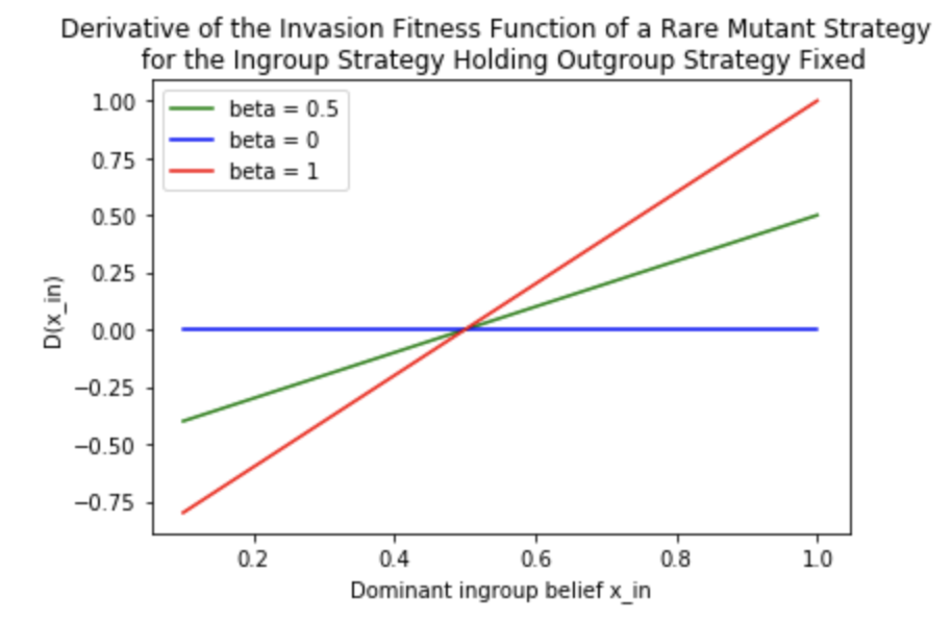
\includegraphics[width=12cm]{images/beta_ingroup_graph}
\end{figure}


\end{document}
